% Presentation (content) for talk at GPN3
% TYPOGRAPHY
% \documentclass[ngerman,handout, usepdftitle=true]{beamer}

\usepackage{fontspec}
\usepackage[shorthands=off]{babel}
\usepackage{csquotes}
\usepackage{graphicx}
\graphicspath{{./images/}}
\usepackage{mathtools}
\usepackage{booktabs}

% fonts for demonstration in LaTeX
% Computer Modern Roman (default); short: cmr

% \usepackage{droidserif} % Antiqua font; short: fdr
\newfontfamily\fontfamilydroidserif{DroidSerif-Regular}

% \usepackage[rm]{roboto} % Slab Serif font; short: RobotoSlab-LF
\newfontfamily\fontfamilyrobotoslab{RobotoSlab-Regular}

% \usepackage[sfdefault]{FiraSans} % Sans Serif font; short: FiraSans-ProportionalLF
\newfontfamily\fontfamilyfirasans{FiraSans-Regular}

% \usepackage{yfonts} % Blackletter fonts (Schwabacher); short: yswab
% or \swabfamily
\newfontfamily\fontfamilyfraktur{UnifrakturMaguntia}
% \newfontfamily\fontfamilyschwabacher{yswab.afm}

% \usepackage{lmodern} % Latin Modern Roman; short: lmr
\newfontfamily\fontfamilylatinmodern{Latin Modern Roman}

\newcommand*{\code}[1]{\texttt{#1}}

% newcommands
\newcommand{\Beispieltext}{%
  \fontsize{5pt}{6pt}\selectfont
  \fontfamilylatinmodern
  Dies ist ein Beispieltext zu möglichem Textsatz.
  Dies ist ein Beispieltext zu möglichem Textsatz.
  Und dies ist noch mehr Beispieltext zu möglichem Textsatz.
  Dies ist ein Beispieltext zu möglichem Textsatz.
  Dies ist ein Beispieltext zu möglichem Textsatz.
  Und noch mehr Beispieltext zu möglichem Textsatz.
  Dies ist ein Beispieltext zu möglichem Textsatz.
  Und dies ist noch mehr Beispieltext zu möglichem Textsatz.
  Dies ist ein Beispieltext zu möglichem Textsatz.
  Und noch mehr Beispieltext zu möglichem Textsatz.
  Dies ist ein Beispieltext zu möglichem Textsatz.
  Dies ist ein Beispieltext zu möglichem Textsatz.
}

% titlepage
\title{Typographie – ein Einblick}
\author{Gesina Schwalbe}

\begin{document}

% title and table of contents
\frame{\maketitle}
\frame{\tableofcontents[hideallsubsections]}

% ------

Dies ist eine Notizensammlung zum zugehörigen Vortrag
\enquote{Typographie – ein Einblick} auf der 3.~GPN der
F3L-Community am 11.06.2016 an der Universität Regensburg.

\section{Was ist Typographie?}
\frame{\sectionpage}
Es gibt durch die historische Entwicklung und heutige Vielfalt der
Anwendung keine klare Definition, was alles Typographie ist, bzw. wo
Typographie aufhört und reines Design anfängt.
Daher ein kurzer Blick auf den kleinsten gemeinsamen Nenner und die
verschiedenen Aspekte, die in der historischen Entwicklung
hinzugekommen sind.

\subsection{Definition}
Hier ein paar gesammelte Definitionen von Typographie: 
\begin{frame}
  \begin{quote}<+->
    Typography is the visual component of the written word. \\
    (\href{http://practicaltypography.com/}{Matthew Butterick})
  \end{quote}
  \begin{quote}<.->
    [Typografie ist die] visuelle Gestaltung eines Druckerzeugnisses,
    eines virtuellen Mediums oder einer dreidimensionalen Oberfläche[.]\\
    (\href{http://www.typolexikon.de/typographie/}{Typolexikon})
  \end{quote}
  \begin{quote}<+->
    Typographie ist visuelle Textgestaltung.\\
    (ich)
  \end{quote}
\end{frame}
Zusammengefasst: Überall, wo geschriebenes Wort zu finden ist, ist
Typographie, d.\,h. Textkomposition!

Der Vortrag soll wegen der Vielfältigkeit von Typographie kein striktes
Erstellmuster für Dokumente liefern. Es wird stattdessen darauf
eingegangen, worauf man beim Erstellen von Textdokumenten überhaupt alles
achten kann und gegebenenfalls für häufige Fälle Umsetzungshinweise
gegeben.


\begin{frame}[t]{Teilbereiche}
  \mode<article>{%
    Typographische Überlegungen lassen sich unterteilen in folgende
    Bereiche, die wir betrachten werden:
  }
  \begin{block}{Mikrotypographie}<1|only@1>
    Details einzelner Zeichen und direkte Beziehungen
    \begin{itemize}
    \item Zeichensetzung
    \item Schriftart
    \item Zeichen-/Wortabstände, Kerning, Ligaturen
    \end{itemize}
  \end{block}
  \begin{block}{Makrotypographie}<2|only@2>
    Layout; Verhältnisse aller Elemente zueinander
    \begin{itemize}
    \item Seitenformat
    \item Satzspiegel, Zeilenbreite
    \item Schriftgröße, Zeilenabstand, Absatzkennzeichnung
    \item Textsatz, Trennung
    \item Hervorhebungen
    \item Zusatzelemente
    \end{itemize}
  \end{block}
\end{frame}

% ---

\subsection{Einfluss von Typographie}
\frame{\subsectionpage}
Der Einfluss von Typographie ist wesentlich weitreichender, als meist
angenommen. Hierzu ein Zitat aus Wikipedia, das es ganz gut beschreibt:

\begin{frame}
  \begin{quote}
    Mithilfe von Typografie kann der Inhalt, Zweck und die Anmutung eines
    Werkes verdeutlicht werden. \\(Wikipedia)
  \end{quote}
\end{frame}

Es gibt viele Situationen, in denen die Darstellung der Inhalte das
Ziel des Schriftstücks ebenso unterstützt, wie deren Qualität.
Daraus folgt auch der wichtigste Punkt vor jeder Überlegung zu
Textsatz/Design/etc. eines Dokuments:
\begin{quote}
  \emph{Was ist der \emph{Zweck} des Dokuments?}
\end{quote}
Das kann (kompetente) Wissensvermittlung genauso wie reine
Aufmerksamkeit, ein Wiedererkennungseffekt oder Wachsamkeit sein.

\begin{frame}{Beispiele für Einflussbereiche von Typographie}
  \begin{description}[Aufmerksamkeit]
  \item[Lesbarkeit] 
    Namenschilder, 
    Verkehrsschilder
  \item[Wachsamkeit] 
    Sicherheitsanweisungen\note{Flugzeugchecklisten}, 
    Dokumentationen\note{NASA}
  \item[Aufmerksamkeit] 
    Bewerbungen,
    Projektanträge,
    Mahnbriefe
  \end{description}
\end{frame}

% ---

\subsection{Historie}
\begin{frame}
  \subsectionpage
  
  \centering
  Wo kommen Gewohnheiten her?
\end{frame}

Diese Frage ist leicht beantwortet: Die meisten Standards, die wir aus
heutigen Dokumenten kennen, haben sich historisch aufgrund technischer
Gegebenheiten etabliert.
Neben Ursprüngen vor Gutenberg stammt Vieles stammt aus der
Schreibmaschinenzeit.
Bedenke also jede typographische Entscheidung (insb. Intuition) und
löse dich von Gewohnheiten, die durch die heutigen Mittel überholt
sind.
\emph{Typographie ist gesunder Menschenverstand.}

\begin{frame}{Ursprüngliche Typographie}
  \mode<article>{Die ursprüngliche Bedeutung von Typographie nach
    Gutenberg lässt sich ganz gut aus einer aktuellen Definition ablesen:}
  \begin{block}{Duden}
    \begin{enumerate}
    \item Kunst der Gestaltung von Druck-Erzeugnissen nach
      ästhetischen Gesichtspunkten; \alert{Buchdruckerkunst}
    \item typografische Gestaltung (eines Druck-Erzeugnisses)
    \end{enumerate}
  \end{block}
\end{frame}

Ganz interessant ist es, sich die Entwicklung einiger Standards im
Laufe der technischen Möglichkeiten anzusehen.
\begin{frame}{Historische Entwicklungen}
  \begin{description}
  \item[Anfänge] Handschrift (kursiv oder gebrochen)\\<article>
    \mode<article>{
      Am Anfang war der Typograph vor allem für den
      Satzspiegel zuständig, Grafiken etc. wurden im Nachhinein
      eingefügt. Zudem war die Schrift vom Schreiber abhängig und
      sollte je nachdem besonders künstlerisch oder platzsparend
      sein.}
  \item[15.\,Jh.] Buchdruck\\<article>
    \mode<article>{
      Erstmals konnten Schriften vereinheitlicht werden und
      die (teuren meist selbst entworfenen) Letternsätze zählten mit
      zu den typographischen Überlegungen.
      Die Serifen in der Schrift wurden beibehalten,
      weil sie die Zeilenorientierung beim Lesen unterstützen.}
  \item[16.\,Jh.] platzsparende Kursivschriften im Druck\\<article>
    \mode<article>{
      Kursive Schriftformen wurden vor allem zum Papiersparen
      eingeführt, sind also nicht leseoptimiert.
      Heutzutage können sie zur Hervorhebung verwendet werden.}
  \item[18.\,Jh] Farbdruck/Lithographie\\<article>
    \mode<article>{
      Erstmals fielen grafische Gestaltungselemente in den Bereich
      der Typographen. Platzierung von Sonderelementen wurde von Belang.}
  \item[1816] Sans Serif\\<article>
    \mode<article>{
      Serifenlose Schriften (auch Grotesk) sind tatsächlich nicht
      sehr alt und ein Produkt der Werbeindustrie. Sie sollten
      auffallen.
      Zu Beginn des Internets wurden sie gerne für Webseiten
      verwendet, weil Serifen bei der damals schlechten
      Bildschirmauflösung keinen Sinn machten.} 
  \item[1870er] Schreibmaschine\\<article>
    \mode<article>{
      Die Schreibmaschine machte Textdokumente und somit Typographie
      zur Massenware.
      Viele Einschränkungen (Monotype-Schriftarten, festgelegter
      Wort-/Zeilenabstand, Leerzeile statt Absatzabstand,
      Unterstreichen zur Hervorhebung etc.) verfolgen uns bis heute.}
  \item[1970er] Markup Sprachen (GenCode, GML; SMGL als erste
    standardisiert)\\<article>
    \mode<article>{
      Die Digitalisierung von Typographie begann mit den
      Markup-Sprachen. Alle digitalen Textdokumente basieren
      hierauf.
    }
  \item[1984] WYSIWYG (Apple mit MacWrite)\\<article>
    \mode<article>{
      \enquote{\textbf{W}hat \textbf{Y}ou \textbf{S}ee \textbf{I}s
        \textbf{W}hat \textbf{Y}ou \textbf{G}et}
      wurde wie der PC von Apple massentauglich gemacht.
      Word-Editoren sind wegen der direkten Rückmeldung sehr
      verbreitet.
      Allerdings darf man hier nicht vergessen, Formatvorlagen zu
      verwenden, um Konsistenz zu wahren!
      Man darf sich zudem nicht ohne einen Gedanken daran mit den
      Defaults zufrieden geben. Diese sind historisch bedingt meist
      auf Papiersparen oder Bildschirmdarstellung optimiert.}
  \item[90er] Internet\\<article>
    \mode<article>{
      Das Internet bzw. der freie Zugang zu Webseiten basierend auf
      HTML und CSS ließ Designbestrebungen explodieren.
      Unglücklicherweise haben die neuen Möglichkeiten die meisten
      Entwickler zu sehr beflügelt, unsinnige und mehr ablenkende
      Grafikelemente einzublenden.
      Die finanzielle Abhängigkeit von Werbung sorgt zudem auf
      vielen Webseiten, insb. denen von Zeitungen, dafür,
      dass statt den Inhalt zu unterstützen möglichst viel davon auf
      Adds abgelenkt wird.
    }
  \end{description}
\end{frame}

\subsection{Zusammenfassung}
\begin{frame}
  \frametitle<presentation>{Zusammenfassung}
  \begin{itemize}
  \item Typographie ist (jede) visuelle Präsentation von Inhalt.
  \item Viele Gewohnheiten sind historisch-technisch, immer überdenken.
  \item Richte Textdarstellung nach dem Zweck des Dokuments.
    \mode<article>{Beachte dabei die Darstellungsform (Druck/Screen, Kontext?).}
  \end{itemize}
\end{frame}

% ------

% \begin{frame}{allgemeine Hinweise}
%   \begin{itemize}
%   \item<1-> Nutze Formatvorlagen (Word/LibreOffice) oder Markup (HTML,
%     LaTeX) für Konsistenz und Wartung.
%   \item<2-> Erst das Ziel, dann der Inhalt, zum Schluss der Satz
%   \end{itemize}
%   \note<2>{Votragsaufbau: vom Detail zum Gesamtbild}
% \end{frame}

\section{Mikrotypographie}
\frame{
  \sectionpage
  
  \centering 
  \mode<presentation>{Details der Zeichen}
}

Mirkotypographie befasst sich grob gesagt mit den Details der Zeichen,
mit denen der Inhalt dargestellt wird. Dazu gehören die Zeichenwahl,
ihr Aussehen (also die Schriftart bzw. Kombination von Schriftarten)
und das Zusammenspiel von kleinen Zeichengruppen (Kerning, Ligaturen).

\subsection{Zeichenwahl}
\frame{\subsectionpage}
\begin{frame}{Die richtigen Zeichen}
  \mode<article>{
    Ein Zeugnis von Professionalität ist es, seine Tastatur zu kennen,
    d.\,h. die richtigen Zeichen (meist UTF-8-Symbole) für einen
    gesuchten Ausdruck zu finden. Im Folgenden ein paar Beispiele.
    Siehe \autoref{tab:zeichen}.
    \begin{table}
      \captionabove{Die richtigen Zeichen wählen
        \label{tab:zeichen}}
    }
    \centering
    \begin{tabular}{llll}
      \toprule
      & Zeichen & Eingabe & so nicht \\\midrule[\heavyrulewidth]
      Ellipsen & … &\code{AltGr+.} 
                          & ...\\\midrule
      Minus, Gedankenstrich, bis & – & \code{AltGr+-} 
                          & - oder ---\\\midrule
      Anführungszeichen & „“ & \code{AltGr+v/b} 
                          & " oder '\\\midrule
      kleine Wortabstände & z.\,B. & \code{\&thinsp;}, \code{\textbackslash,}
                          &\\\bottomrule
    \end{tabular}
    \mode<article>{\end{table}}
\end{frame}

\begin{frame}{Die richtigen Umbrüche}
  \mode<article>{
    Für Umbrüche gilt dasselbe wie für jedes andere Zeichen: Wähle die
    richtige Darstellungsform.
    Ein Absatzumbruch ist kein doppelter Zeilenumbruch und richtige
    automatische Worttrennung funktioniert nur mit den entsprechenden
    Hilfszeichen. Siehe \autoref{tab:umbrueche}
    \begin{table}
      \captionabove{Die richtigen Umbrüche/Leerzeichen wählen
        \label{tab:umbrueche}}
    }
    \centering
    \begin{tabular}{lll}
      \toprule
      & Eingabe & so nicht\\\midrule[\heavyrulewidth]
      Zeilenumbruch & \code{Shift+Enter}, \code{<br/>}
                & kein Absatzumbruch\\\midrule
      Absatzumbruch (¶)& \code{Enter} 
                & keine Leerzeile(n)\\\midrule
      Seitenumbruch &
                & keine 1000 Leerzeilen\\\midrule
      geschütztes Leerz. & \code{Strg+Shift+Leer}%, \code{\&nbsp;}
                & „1. Sep.“ trennen \\\midrule
      weiches Trennz. & \code{Strg+-}, \code{\&shy;}
                & \\\bottomrule
    \end{tabular}
    \mode<article>{\end{table}}
\end{frame}

% ---

\subsection{Schrift}
\frame{
  \subsectionpage

  CSS: \code{font-family: <schriftart>;}
}

Die Schrift stellt einen großen Anteil der Wirkung und Lesbarkeit
eines Textes. Daher eine Einführung, welche Schriftarten es gibt,
in welchen Situationen sich welche gut machen und warum.
Wir beginnen mit verschiedenen Unterteilungen und Begrifflichkeiten.

\begin{frame}{Schriftfamilien}
  \mode<article>{Vorweg der Unterschied von Schriftart und
    Schriftfamilie (was heute meist als Schriftart bezeichnet wird):}
  \begin{description}[Schriftfamilie]
  \item[Schriftart] ein Zeichensatz in best. Schnitt 
    (z.\,B. Latin Modern Roman Slanted)
  \item[Schriftfamilie] Sammlung zusammengehöriger Schriftarten
    (kursiv, grotesk, monotype, untersch. Schnitte, Kapitälchen)
  \end{description}
\end{frame}

\begin{frame}{Schriftgattungen}
  \mode<article>{
    Die Schriftgattung ist die gröbste Unterteilung von Schriften.
    Hier ein Europäisches Gattungssystem:
  }
  \begin{block}{Antiqua}
    rundbogige lateinische Schriften\\<article>
    \mode<article>{
      Diese Schriften haben sich mit dem Buchdruck entwickelt.
      Sie sind die häufigsten (römischen) Schriften.
    }
  \end{block}
  \begin{block}{Gebrochene Schriften}
    mittelalterliche Frakturschriften, z.\,B.\\<all>
    {\fontfamilyfraktur dieser Text ist geschrieben in Unifraktur
      Maguntia.}
    \\<article>
    \mode<article>{
      Frakturschriften kommen aus der handschriftlichen Zeit, in der
      mit Federkielen geschrieben wurde. Aufgrund der breiten Federn
      war der bruchartige Richtungswechsel beim Schreiben unumgänglich
      für den Schreibfluss. Aus den kunstvollen Strichabschlüssen
      wurden im Druck die Serifen.
    }
  \end{block}
  \begin{block}{Nichtrömisch}
    Griechisch, Kyrillisch, Arabisch, Chinesisch …
  \end{block}
\end{frame}

\begin{frame}{Untergruppen der Antiqua}
  \mode<article>{
    Nachdem die Schriftgattung der Antiqua die eigentlichen
    Druckschriften ausmacht, hier näheres dazu.
    (Tipp: Es macht nur in ganz seltenen Fällen Sinn, gebrochene
    Schriften zu verwenden. Sie sind meist schlecht als Fließtext
    lesbar. Dafür vermitteln sie einen kalligraphischen Eindruck.)
  }
  \begin{block}{Antiqua}<+->
    dreieckige Serifen\\<all>[2pt]
    {\fontfamilydroidserif Dieser Text ist geschrieben in Droid
      Serif.}\\<all>
    {\fontfamilylatinmodern Dieser Text ist geschrieben in Latin
      Modern.}\\<article>
    \mode<article>{
      Serifenschriften haben den großen Vorteil, dass Serifen die
      Zeilenorientierung unterstützen. Antiqua Serifenschriften
      sind meist zusätzlich auf Eleganz und Grauwert (Schwarzwirkung
      der Schrift) optimiert.
    }
  \end{block}
  \begin{block}{Egyptienne}<+->
    auch \emph{serifenbetonte Linear-Antiqua}; 
    betonte Serifen, glm. Dicke\\<all>
    {\fontfamilyrobotoslab Dieser Text ist geschrieben in Roboto Slab.}\\<article>
    \mode<article>{
      Diese Serifenschriften erweisen sich oft als vorteilhaft bei
      schlechter Bildschirmauflösung, da sie keine schmalen Stege
      haben wie die meisten Antiqua und die Serifen betonter sind.
      Sie wurden ursprünglich für Werbeanzeigen entwickelt.
    }
  \end{block}
  \begin{block}{Grotesk (Sans Serif)}<+->
    serifenlos\\<all>
    {\fontfamilyfirasans Dieser Text ist geschrieben in Fira Sans.}\\<article>
    \mode<article>{
      Serifenlos haben kein Problem mehr mit schlechter
      Bildschirmdarstellung, sind daher historisch beliebt für
      Webseiten. Diese Zeit ist jedoch vorbei und serifenlos sollte
      bei viel Fließtext eher vermieden werden. Dafür bietet es eine
      gute Hervorhebungsmöglichkeit für z.\,B. Überschriften in
      Kombination mit Antiqua/Egyptienne Textkörper.
    }
  \end{block}
\end{frame}

\begin{frame}[t]{Worauf kann man achten?}
  \mode<article>{
    Die Wahl der Schrift ist nicht so einfach, deshalb hier ein paar
    Anhaltspunkte, worauf man achten kann. Wichtig dabei ist, dass man
    \emph{erst den Hauptteil} (abhängig vom Zweck, meist der
    Textkörper) betrachtet, dann die Zusatzelemente
    (z.\,B. Überschriften, Auflistungen, Zitate, …).
    Die Auflistung ist in etwa absteigend nach Relevanz sortiert.
  }
  \mode<presentation|uncover@+->{Immer zuerst Aussageteil (meist Textkörper)!}
  \begin{block}{Schriftgruppe}<+-|only@-4>
    mit/ohne Serifen (kein Monotype außer für Code)
    \begin{itemize}
    \item Viel Text: Serifen unterstützen Zeilenorientierung
    \item Schlechte Auflösung: Serifenlos meist besser dargestellt
      \note<.>{Deshalb sind Serifen im Netz so häufig; früher war die
        Bildschirmqualität i.\,A. schlecht.}
    \end{itemize}
  \end{block}
  \begin{block}{Grauwert}<+-|only@-4>
    Flächendeckung der Schrift; betrachte versch. Schnitte\\
    \mode<presentation>{Screen mehr, Druck weniger}
    \mode<article>{
      \begin{itemize}
      \item Bildschirm: eher mehr Grauwert 
        (und weniger Kontrast, falls selbstleuchtend)
      \item Druck: eher weniger Grauwert
      \end{itemize}
    }
  \end{block}
  \begin{block}{Qualität}<+-|only@-4>
    Detailreichtum der Schrift
    \mode<article>{variiert teilw. recht start;
      Zum Feststellen der Qualität am besten am Bildschirm
      heranzoomen.
      Grundsätzlich sind bessere (konsistent und professionell wirkende)
      Schriften zu bevorzugen.}
  \end{block}
  \begin{block}{Features}<+-|only@+->
    OpenType Features bei OTF\mode<article>{(=\textbf{O}pen
      \textbf{T}ype \textbf{F}ont)}
    (Kapitälchen, Ligaturen, Kerning, Alternative Zahlen …)
  \end{block}
  \begin{block}{Weite}<+-|only@+->
    Wie dicht ist die Schrift?
    \mode<article>{Schriften sind unterschiedlich weit, brauchen also
      entsprechend mehr oder weniger Platz im Druck.
      Ein Beispiel einer dichten Schrift ist Times New Roman, das für
      die namensgebende Zeitung entwickelt wurde.}
  \end{block}
  \begin{block}{Wirkung}<+-|only@+->
    Modern/gediegen? Seriös/lustig?
    \mode<article>{Hierbei ist zu beachten, dass viele Systemschriften
      (Times New, Helvetica, Verdana, Arial, …) aufgrund ihrer
      Häufigkeit unseriös wirken. Computer Modern und ähnliche
      Standardschriften für Fachzeitungen wiederum sind im Allgemeinen
      mit Seriosität konnotiert.}
  \end{block}
  \begin{block}{Kosten}<+-|only@+->
    \mode<article>{Eine Schrift zu entwickeln mit allen Features kostet
      viel Zeit und Erfahrung. Entsprechend kosten professionelle
      Schriften(/-familien) meist ab 100 Euro aufwärts.}
  \end{block}
\end{frame}

\begin{frame}{Schriften vergleichen}
  \mode<presentation>{gleichen Text auf selbe Höhe bringen,
    vergleichen\par\vfill}
  \mode<article>{Um Schriften nachhaltig miteinander zu vergleichen,
    sollte man auf jeden Fall einen längeren Textabsatz verwenden.
    Dann sollten sie auf \emph{dieselbe Höhe} (nicht Breite) gebracht
    werden und der \emph{Zeilenabstand} entsprechend für jede Schrift
    einzeln angepasst werden. 
    Dann sollte man auch verschiedene Medien zur Ansicht verwenden, um
    optimale \emph{Verwendungsbereiche} festzustellen:
    \begin{itemize}
    \item Bildschirm (evtl. hohe und geringe Auflösung)
    \item Tintenstrahldrucker
    \item Laserdrucker
    \end{itemize}
  }
  \begin{exampleblock}{Beispiel}<+->
    S. \href[pdfnewwindow=true]{./examples/fonts.pdf}%
    {Beispieldokument mit Schriftvergleich freier Schriften}
    %% Example
    % fonts.pdf
  \end{exampleblock}
\end{frame}

\begin{frame}{Mischen von Schriften}
  \mode<article>{Beim Mischen von Schriften, was insbesondere nötig
    ist, wenn die gewünschte Schrift keine zugehörige Schriftfamilie
    anbietet, ist zumindest zu beachten:}
  \begin{alertblock}{Nicht zu viele versch. Schriftfamilien}
    Stiftet Verwirrung und Schriftdateien werden eingebettet%
    \mode<article>{, was zu unnötiger Dateigröße führt.}
  \end{alertblock}
  \begin{alertblock}{Auf Konsistenz achten}
    Erst die Hauptschriftart und die anderen daran orientiert%
    \mode<article>{ auswählen.}
  \end{alertblock}
\end{frame}

% ---

\subsection{Zeichengruppen}
\frame{\subsectionpage}
Hier werden zwei Möglichkeiten vorgestellt, wie man das
Erscheinungsbild einzelner Zeichengruppen verbessern kann.

\begin{frame}{Kerning}
  \mode<article>{Kerning ist das Anpassen des Zeichenabstands (und damit
    auch -überstands in einigen Fällen) zwischen einzelnen
    Zeichenpaaren. Für ein Beispiel siehe \autoref{fig:kerning}.
    Es ist ein OpenType-Feature und muss meist manuell aktiviert
    werden.
    \begin{figure}
      \centering
      
\includegraphics[width=3cm]{Kerning_without.png}\\
      
\includegraphics[width=3cm]{Kerning_with.png}\\
      \caption{Zwei Beispiele für Kerning\label{fig:kerning}}
    \end{figure}
  }
  \mode<presentation>{Anpassen des Zeichenab-/überstands bei
    best. Zeichenpaaren
    \begin{center}
      
\includegraphics[height=.2\paperheight]{Kerning_without.png}
      
\includegraphics[height=.2\paperheight]{Kerning_with.png}
    \end{center}
    \vfill}
  CSS:\\ 
  \code{text-rendering: optimizeLegibility; \\<all>
    <browser-prefix>font-feature-settings: kern;}
\end{frame}

\begin{frame}{Ligaturen}
  \mode<article>{%
    Eine Ligatur ist der Verbund mehrerer Buchstaben zu einem
    Zeichen. Neben Designüberlegungen (z.\,B. ist \& eine Ligatur),
    ist ein häufiger praktischer Grund, dass Zeichen ohne Ligatur zu
    weit auseinander stehen und mit Körning an einigen Stellen
    überlappen würden. Für ein Beispiel siehe \autoref{fig:ligature}
    Ligaturen sind auch OpenType-Features (sie werden als eigene
    Zeichen abgespeichert) und müssen meist manuell eingeschaltet
    werden.
    \begin{figure}
      \centering
      
\includegraphics[width=3cm]{Ligatures.png}
      \caption{Zwei Beispiele für Ligaturen\label{fig:ligature}}
    \end{figure}
  }
  \mode<presentation>{%
    Buchstabenverbund für schönere Abstände/Überlappungen
    \begin{center}
      
\includegraphics[height=.2\paperheight]{Ligatures.png}
    \end{center}
    \vfill
  }
  CSS: \code{text-rendering: optimizeLegibility;}  
\end{frame}

% ---

\subsection{Zusammenfassung}
\begin{frame}
  \frametitle<presentation>{Zusammenfassung}
  \begin{enumerate}
  \item Inhalt richtig eingeben
  \item Schrift auswählen anhand von 
    \begin{itemize}
    \item Darstellungsmedium ($\Rightarrow$ Serifen, Grauwert, Weite)
    \item Wirkung
    \item Qualität, Features
    \end{itemize}
  \item Features nutzen (Kerning, Ligaturen, etc.)
  \end{enumerate}
\end{frame}

% ------

\section{Makrotypographie}
Mit Makrotypographie ist jede visuelle Gestaltung des Gesamtbildes
gemeint. Also nicht mehr einzelne Zeichen oder Zeichengruppen, sondern
ganze Absätze, Textblöcke, Hervorhebungen, eingebundene Grafiken etc.
Hier wird von den wichtigen Teilen (Erscheinungsbild des Textkörpers)
zu den Sonderelementen (Hervorhebungen und Grafiken) gegangen und jeweils
erst die essenziellen, dann die weniger wichtigen Überlegungen
anführt.
Wie bisher ist das nicht als strikte Anleitung zu sehen, sondern als
Sammlung von Punkten, über die man sich Gedanken gemacht haben sollte
bzw. Gedanken machen kann.

\begin{frame}<presentation>
  \sectionpage
  \centering
  Das Gesamtbild
  \note{Von wichtigen Teilen (Textkörper) zu unwichtigen (Metadaten, Hervorhebungen)
    Von Essentiellem zu Ästhetik}
\end{frame}

\subsection{Layout}
Zu Beginn sollte die Grobstruktur optimiert werden. Diese macht im
Normalfall einen Großteil des Gesamteindrucks aus. Hierzu tragen
Satzspiegel, damit verbunden der Grauwert und die Strukturierung von
Elementen (z.\,B. Absätzen) bei.
\begin{frame}<presentation>
  \subsectionpage
  \centering
  essentielle Überlegungen: \\
  ersten Eindruck festlegen 
  mit \emph{Grauwert} und \emph{Grobstruktur}
\end{frame}

\begin{frame}{Schrift-/Hintergrundfarbe}
\mode<article>{Hier ist wieder wie immer der Zweck des Dokuments
  einzubeziehen. Aber generell gilt: Der Hintergrund ist dafür da, den
  Vordergrund (also den wichtigen Informationsträger) lesbar zu
  machen.
  Dementsprechend nicht mit dem Hintergrund z.\,B. durch
  kontrastreiche Bilder vom Text ablenken.}
  \begin{block}{Druck}<+->
    \begin{itemize}
    \item möglichst hoher Kontrast%
      \mode<article>{, da Papier passiv leuchtend ist.}
    \item schwarz auf Weiß (Kosten)
    \end{itemize}
  \end{block}
  \begin{block}{Screen, Beamer}<+->
    \begin{itemize}
    \item Kontrast verringern (Bildschirme leuchten aktiv)
    \item keine irritierenden/beißenden Farben
    \end{itemize}
  \end{block}
\end{frame}

\begin{frame}{Schriftgröße}
  \mode<article>{Die Schriftgröße beeinflusst (auch bei vergrößerbaren
    Medien!) wesentlich die Leserlichkeit und den ersten Eindruck
    davon.
    Zu große Schrift wird von Nahem durch den großen
    Betrachtungswinkel auch schwer lesbar.
    Bei den Überlegungen sollte also immer der voraussichtliche
    Abstand beim Lesen mit eingerechnet werden
    (Plakat$\neq$Visitenkarte).
    Bewährt haben sich folgende Werte:
  }
  \begin{description}[Screen (insb. Web)]
  \item[Druck] 10–12pt (kurze Lesedistanz)
  \item[Screen (insb. Web)] 15–20px
        \mode<article>{(meist weiter vom Bildschirm entfernt beim
          lesen – denke aber an mobile Geräte!)}
  \item[Präsentation] nicht zu klein
    \mode<article>{(Wo wird der Vortrag gehalten?)}
  \end{description}
  \mode<presentation>{\vfill}
  CSS: \code{font-size: …px}
\end{frame}

\begin{frame}{Zeilenabstände}
  Faustregel: 120–140\% der Schriftgröße%
  \mode<article>{; das haut bei den gängigen Schriften hin.
    Trotdem geht nichts über ausprobieren.
    Hierbei beachten: Kleine Änderungen können viel an der Wirkung
    ändern; ich empfehle im 5\%-Bereich herumprobiert zu haben.
    }
  \mode<presentation>{
    \begin{columns}[onlytextwidth,T]
      \begin{column}{.3\paperwidth}
        \fontsize{8pt}{8.8pt}\selectfont
        \fontfamilylatinmodern
        110\%:
        Dies ist ein Beispiel für Abstände zwischen Zeilen.
        Dies ist ein Beispiel für Abstände zwischen Zeilen.
        Dies ist ein Beispiel für Abstände zwischen Zeilen.
        Dies ist ein Beispiel für Abstände zwischen Zeilen.
      \end{column}
      \begin{column}{.3\paperwidth}
        \fontsize{8pt}{10.4pt}\selectfont
        \fontfamilylatinmodern
        130\%:
        Dies ist ein Beispiel für Abstände zwischen Zeilen.
        Dies ist ein Beispiel für Abstände zwischen Zeilen.
        Dies ist ein Beispiel für Abstände zwischen Zeilen.
        Dies ist ein Beispiel für Abstände zwischen Zeilen.
      \end{column}
      \begin{column}{.3\paperwidth}    
        \fontsize{8pt}{13.6pt}\selectfont
        \fontfamilylatinmodern
        170\%:
        Dies ist ein Beispiel für Abstände zwischen Zeilen.
        Dies ist ein Beispiel für Abstände zwischen Zeilen.
        Dies ist ein Beispiel für Abstände zwischen Zeilen.
      \end{column}
    \end{columns}
    \vfill}
  CSS: \code{line-heigt: 1.3} (ohne Einheit)
\end{frame}

\begin{frame}{Absatzabstände}
  \mode<article>{Absätze sind eigenständige Textelemente (meist
    Sinnabschnitte), die für die Verständlichkeit entsprechend
    gekennzeichnet werden müssen. Hierzu haben sich historisch
    Absatzabstand oder Einzug etabliert. Andere Möglichkeiten
    (Trennzeichen/-linien etc.) sind meistens zu auffällig für diesen
    Zweck, siehe Hervorhebungen. Also:}
  \begin{itemize}
  \item Abstand \alert{oder} Einzug (\alert{keine} Leerzeile)
    \begin{description}
    \item[Abstand] 50–100\% der Schriftgröße\\<all>
      CSS: \code{p \{margin-bottom: 0.75;\}}
    \item[Einzug] 1–4em (1em $\approx$ Schrifthöhe)\\<all>
      CSS: \code{p \{text-indent: …em;\}} \note{em wird in px umgerechnet}
    \end{description}
  \item Schusterjungen und Hurenkinder verhindern
  \end{itemize}
\end{frame}

\begin{frame}{Satzspiegel}
  \mode<article>{Der Satzspiegel ist die Aufteilung in
    Textbereich/Vordergrund und Rand/Hintergrund (oder mehr
    Ebenen). Wichtig: Orientiere dich immer am eigentlichen
    Textkörper/Inhalt!}
  \begin{itemize}[<+->]
  \item max. Zeilenbreite 2–3 Alphabete\\
    \mode<article>{sonst geht der Zeilenbezug verloren}
    abcdefghjklmnopqrstuvwxyzabcdefghjklmnopqrstuvwxyz
  \item evtl. mehrere Spalten\\(nicht zu viele!)
  \item genügend Rand\\
    \mode<article>{für Ausgleich im Grauwert;
      Der Grauwert ist sehr wichtig für den ersten
      Eindruck und wird wesentlich vom Verhältnis von Rand zu Schrift
      bestimmt. Also auch bei kleinen Dokumenten (Flyer,
      Visitenkarten, …) genügend Rand lassen.}%
    \mode<presentation>{(Grauwert)}
  \item Textbereich sinnvoll platzieren\\
    (einseitig: zentriert, doppelseitig: innen)
  \end{itemize}
\end{frame}

\begin{frame}{Beispiel Satzspiegelkonstruktion}
  \mode<article>{Satzspiegelkonstruktionen haben sehr lange Tradition,
    da sie bereits für handschriftliche Dokumente nötig waren. Sie
    lassen sich meistens in der Größe des Randes variieren. Man sollte
    sich eine Faustregel für Textdokumente merken, da die meisten
    Word-Editoren eine Voreinstellung mir zu knappem Rand haben
    (rein papiersparend).
    Die Rasterteilung unterteilt längs und quer in (hier) 9 Teile und
    überlässt dem Textbereich $6\times6$ davon, siehe
    \autoref{fig:rasterteilung}. Hierbei die Bindekorrektur nicht
    vergessen!
    \begin{figure}
      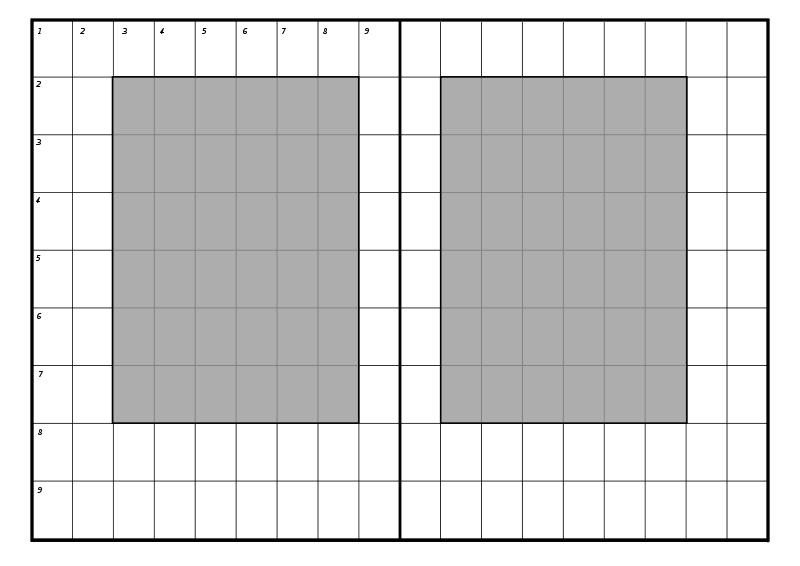
\includegraphics[width=\textwidth]{Satzspiegel-Rasterteilung.png}
      \caption{9er Rasterteilung\label{fig:rasterteilung}}
    \end{figure}
  }
  \mode<presentation>{
    Für begrenzte Textfläche z.\,B.
    \begin{block}{Rasterteilung}
      \centering
      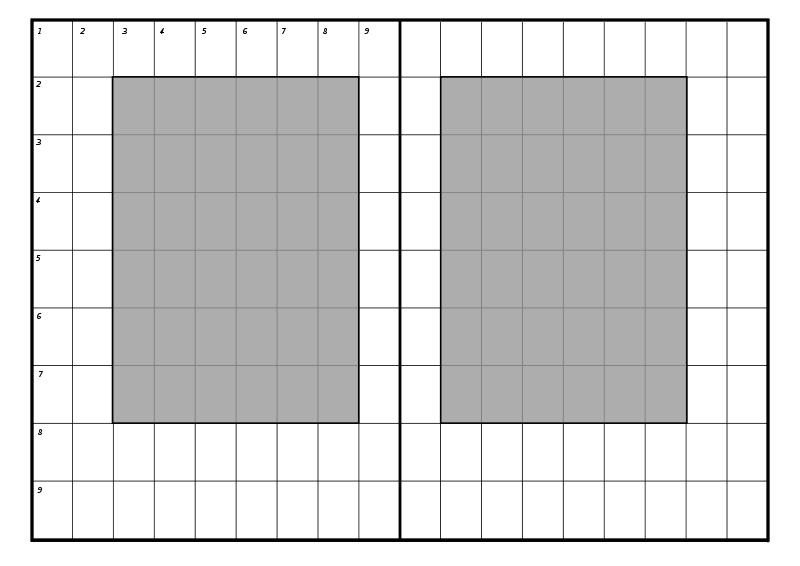
\includegraphics[height=.6\textheight]{Satzspiegel-Rasterteilung.png}
    \end{block}
    Bindekorrektur nicht vergessen!}
\end{frame}

  
\subsection{Textausrichtung}
Die üblichen Textausrichtungen (links-/rechtsbündig,
zentriert oder Blocksatz) sind aus den Word-Editoren bekannt,
allerdings meist nicht richtig oder aus dem richtigen Grund
verwendet. Mit der Schreibmaschine war aufgrund der Monotype-Schrift
nur linksbündig möglich. Rechtbündig und zentriert kamen als
Stilmittel mit der Digitalisierung hinzu während für professionellen
Druck heutzutage Blocksatz verwendet wird. Für ein gleichmäßiges
Aussehen des Textkörpers ist Blocksatz am besten. Allerdings ist er
ungeeignet ohne die richtigen Hilfsmittel der Worttrennung, denn
Blocksatz basiert auf leichtem Dehnen der Wortabstände.

\begin{frame}{Textausrichtung – Grundsätzliches}
  \mode<article>{Hier die grundsätzlichen Überlegungen zur
    Textausrichtung.}
  Zu vermeiden
  \begin{itemize}
  \item (ungleichmäßiger) Flatterrand
  \item zu großer (autom.) Wortabstand
  \end{itemize}
  \mode<presentation>{
    \begin{columns}[T]
      \begin{column}{.3\paperwidth}
        \mode<article>{Linksbündig\par}
        \parbox[t]{\textwidth}{\raggedright\Beispieltext}
      \end{column}
      \begin{column}{.3\paperwidth}
        \mode<article>{Blocksatz\par}
        \parbox[t]{\textwidth}{\Beispieltext}
      \end{column}
      \begin{column}{.3\paperwidth}
        \mode<article>{zentriert\par}
        \parbox[t]{\textwidth}{\centering\Beispieltext}
      \end{column}
    \end{columns}
  }
  % Examples
  % riesenueberschrift.pdf
\end{frame}

\begin{frame}{Textsatz – Empfehlungen}
  \mode<article>{Hier ein paar Empfehlungen, wann man welchen Satz in
    Erwägung ziehen sollte.}
  \begin{description}[schmal/keine Trennung]
  \item[breit]  Worttrennung einschalten, Blocksatz
    \mode<article>{(Blocksatz \emph{nur} mit Worttrennung, sonst
      werden die Wortabstände zu sehr gedehnt!)}
  \item[schmal/keine Trennung] Linksbündig
    \mode<article>{(Dies gilt auch für Webseiten, d.\,h. HTML)}
  \item[nur kurze Passagen] Zentriert%
    \mode<article>{; zentrieren ist aufgrund der Symmetrie ein
      Stilmittel, das z.\,B. für Gedichte angebracht ist, allerdings
      für längere Texte zu wenig Zeilenorientierung bietet, was das
      Lesen anstrengend macht.}
  \item[mögl. nie im Textkörper] Rechtsbündig%
    \mode<article>{; Es ist wie zentriert ein Stilmittel, das zu wenig
      Zeilenorientierung für lange Texte in Sprachen bietet, die man
      von links nach rechts liest.}%
    \mode<presentation>{ (Zeilenorientierung geht verloren)}%
  \end{description}
\end{frame}

\begin{frame}{Worttrennung}
  \mode<article>{Worttrennung ist für Blocksatz unerlässlich aber auch
    sonst platzoptimierend und praktisch. Automatische Worttrennung
    also wenn möglich immer einschalten. Beachte: Trennstriche niemals
    (mit oder ohne automatische Trennung) selbst eingeben, sondern die
    Zeichen für optionale Umbruchstellen verwenden:}
  \mode<presentation>{Benutzen!}
  \begin{description}[--]
  \item[optionale Umbruchstellen]
    LibreOffice: \code{Strg+-}, HTML: \code{\&shy;}
  \item[geschützte Leerzeichen/Bindestriche] insb. bei
    E-Mail-/Webadressen;\\
    LibreOffice: \code{Strg+Shift+Leer}, HTML: \code{\&nbsp;}
  \item[Zeilenumbruch] bei Überschriften etc. manuell einfügen;\\
    LibreOffice: \code{Shift+Enter}, HTML: \code{<br/>}
  \end{description}
  \mode<presentation>{\vfill}
  CSS: \code{hyphens: auto;} (magere Unterstützung)

  \begin{exampleblock}{Beispiel für Notwendigkeit}<2->
    Schmale Spaltenbreite oder
    \href[pdfnewwindow]{./examples/hyphenation.pdf}{lange Wörter}.
  \end{exampleblock}
\end{frame}

\subsection{Hervorhebungen}
Für Hervorhebungen gilt grundsätzlich
\begin{quote}
  Weniger ist mehr.
\end{quote}
Ist zu viel hervorgehoben, hat es keinen Effekt mehr. Hervorhebung
sollte (dezent) für Gliederung und für essentielle
Stichpunkte/Aussagen verwendet werden. Möglichst keine längeren
Passagen hervorheben.
Zusammengefasst:
\begin{quote}
  Wer zu viel schreit, dem hört keiner mehr zu.
\end{quote}
Übrigens sind Ausrufezeichen wegen ihrer Konnotation ebenfalls eine
Form der Hervorhebung einer Aussage. Diese in formalen Texten auch
möglichst selten verwenden.

\begin{frame}<presentation>
  \subsectionpage
  \centering
  Weniger ist mehr, überdecke den Inhalt nicht
\end{frame}

\begin{frame}{So nicht hervorheben}
  \alert<presentation><+->{Generell: Möglichst wenig hervorheben}
  \begin{alertblock}{Nicht unterstreichen!}<+->
    \begin{itemize}
    \item Schreibmaschinen-Gewohnheit
    \item \underline{Unterstreichen ist mit billig} konnotiert
    \end{itemize}
  \end{alertblock}
  \begin{alertblock}{Nicht zu viele Farben!}<+->
    \fontsize{14pt}{18pt}\selectfont
    \frame{\fcolorbox{cyan}{black}{
        \color{red}Zu \color{green}viele
        \color{yellow}kontrastierende
        \color{blue}Farben
        \color{pink}lenken
        \color{magenta}ab!
      }}
  \end{alertblock}
  \begin{exampleblock}{Beispiel}
    \href[pdfnewwindow]{./examples/hervorhebungen.pdf}{So} nicht.
  \end{exampleblock}
\end{frame}

\begin{frame}[t]{Hervorheben im Fließtext}  
  \mode<article>{
    Im Fließtext gibt es u.\,a. folgende übliche Möglichkeiten: Kursiv,
    Fett, Kapitälchen, Farbe, und – bitte nicht –
    Unterstreichen/Versalien (beide aus Schreibmaschinenzeiten).
    Ein paar Kommentare:}
  \begin{block}{\itshape Kursiv}<+-|only@+-3>
    \begin{itemize}
    \item im \textit{Fließtext} zu bevorzugen
    \item bei \textit{Grotesk} meist zu schwach
    \end{itemize}
  \end{block}
  \begin{block}{\bfseries Fett}<+-|only@+-3>
    \begin{itemize}
    \item sehr \textbf{auffällig} durch Kontrast
    \item \textbf{Abstufungen} beachten
      \mode<article>{(oft gibt es neben bold und normal auch
        semibold und weitere Zwischenstufen)}
    \end{itemize}
  \end{block}
  \begin{block}{\scshape Kapitälchen}<+-|only@+-3>
    \begin{itemize}
    \item etwa wie fett, meist \textsc{schwerer lesbar}
      \mode<article>{(Es fehlt das gewohnte Höhenmuster der
        Kleinbuchstaben)}
    \item nur gute verwenden: \textsc{Grauwert} oft zu schwach
      \mode<article>{bei den automatisch erzeugten}
    \end{itemize}
  \end{block}
  \begin{block}{\uppercase{Versalien}}<+-|only@+-5>
  \mode<article>{Versalien stammen aus der Schreibmaschinenzeit und
    werden heute eher als aufdringliches Geschrei bei Vorkommen im
    Fließtext empfunden. Wenn möglich, auf richtige Kapitälchen
    ausweichen.}
    \begin{itemize}
    \item \uppercase{sehr} auffällig, \uppercase{schwer lesbar}
    \item auf \uppercase{Zeichenabstand} achten
    \item \uppercase{nicht} mit Capslock
    \end{itemize}
  \end{block}
  \begin{block}{Farbe}<+-|only@+-5>
    \begin{itemize}
    \item {\color{green}Kontrast} hängt vom Grauwert ab – ausprobieren
    \item auf {\color{green}Konsistenz} achten 
      (nicht zu viele kontrastierende)
    \item Druckkosten\mode<article>{ im Druck beachten (und hier ein
        Farbschema wählen, das der Drucker versteht)}
    \end{itemize}
  \end{block}
  \begin{alertblock}{Beachte:}<+-|only@6>
    Oft sind \emph{Emphasize}-Umgebungen/-Vorlagen
    gegeben:
    \begin{description}
    \item[LibreOffice] Character-Styles
    \item[HTML] \code{<emph>}
    \item[\LaTeX] \code{\textbackslash emph}
    \end{description}
    \mode<article>{
      Für Fließtext sind diese Hervorhebungen im Normalfall völlig
      ausreichend. Außerdem können sie einheitlich umdefiniert werden,
      wenn man eine bessere Methode findet.}
  \end{alertblock}
\end{frame}

\begin{frame}{Sonstiges Hervorheben}
  \begin{block}{Weißraum}<+->
    \mode<article>{Weißraum ist vertikaler oder horizontaler
      Abstand. Dieser ist mit Maß eingesetzt eines der besten Mittel
      für Hervorhebung von Gliederungselementen (vgl. Absatzabstände).
      Einrücken immer wenig, da sonst die Zeilenorientierung wieder
      verloren geht.
      Zusammengefasst: In der Typographie gilt ebenfalls das Prinzip
      \begin{quote}
        Reden ist Silber, Schweigen ist Gold.
      \end{quote}}
    \mode<presentation>{(vertikaler Abstand/Einrücken)\\
      \emph{Reden ist Silber, Schweigen ist Gold.}}
  \end{block}
  \begin{block}{Schriftgröße}<+->
    {\Large kleinstmögliche} erkennbare Schritte machen
    \note<.>{schlechtes Beispiel: HTML-Default der Überschriften}
  \end{block}
  \begin{block}{Rahmen (z.\,B. Code-Blocks)}<+->
    \begin{itemize}
    \item nicht zu auffällig in Dicke/Effekt (überdeckt umrahmtes!)
    \item nicht zu dünn (digital nicht darstellbar)
    \end{itemize}
    \fbox{CSS: \code{border}}
  \end{block}
\end{frame}

\begin{frame}<presentation>{Hervorheben}
  \centering
  \emph{Grundsätzlich:~}

  \vspace*{1.5\baselineskip}
  Weniger ist mehr\\ – \\
  kleinstmögliche Hervorhebung\\
  für den gewünschten Effekt nutzen
\end{frame}


\subsection{Sonderelemente}
Mit Sonderelementen sind hier alle Elemente, die nicht dem Fließtext
angehören, gemeint. Beispielhaft werden hier Tabellen, Formeln,
Grafiken und Briefköpfe behandelt. Überschriften und andere reinen 
Gliederungselemente sollten streng genommen auch dazu gehören, sind
aber unter Hervorhebungen schon ausreichend behandelt worden.
\begin{frame}<presentation>
  \subsectionpage
  \centering
  = Alles außer Fließtext – ein paar Beispiele
\end{frame}

\begin{frame}{Tabellen}
\mode<article>{Tabellen wurden zur Schreibmaschinenzeit mit
  Tabulatoren gesetzt – heute stehen in allen mir bekannten
  Textsatzprogrammen/-sprachen bessere Möglichkeiten. Allerdings sind
  die Defaults meist schlecht lesbar: Zu viele (teils den
  Lesefluss/Datenzusammengehörigkeit störende) Rahmen und zu geringe
  Abstände sind häufig.}
  \begin{block}{Rahmen}
    nicht zu auffällig; Steigerung:
    \begin{enumerate}
    \item nur Trennlinien (oben, unten)
    \item horizontale
    \item vertikale
    \end{enumerate}
    CSS: \code{border-width}, \code{border}
  \end{block}
  \begin{block}{Abstände}
    CSS: \code{padding}
  \end{block}
\end{frame}

\begin{frame}{Tabellen – Vergleich}
  \begin{description}
  \item[zu viel]~
    \parbox[t]{.5\textwidth}{
      \fontsize{8pt}{10.4pt}\selectfont
      \begin{tabular}{|l|c|l|}
        \hline
        Bezeichnung & Zeichen & UTF-8\\\hline
        Hyphen Minus & - & \code{U+002D}\\\hline
        En Dash & – & \code{U+2013}\\\hline
        Em Dash & --- & \code{U+2014}\\\hline
      \end{tabular}
      \\[\baselineskip]\mbox{}}

  \item[in Ordnung]~
    \parbox[t]{.5\textwidth}{
      \fontsize{8pt}{10.4pt}\selectfont
      \begin{tabular}{lcl}
        \toprule
        Bezeichnung & Zeichen & UTF-8\\\midrule[\heavyrulewidth]
        Hyphen Minus & - & \code{U+002D}\\\midrule
        En Dash & – & \code{U+2013}\\\midrule
        Em Dash & --- & \code{U+2014}\\\bottomrule
      \end{tabular}
      \\[\baselineskip]\mbox{}}

  \item[reicht völlig]~
    \parbox[t]{.5\textwidth}{
      \fontsize{8pt}{10.4pt}\selectfont
      \begin{tabular}{lcl}
        \toprule
        Bezeichnung & Zeichen & UTF-8\\\midrule[\heavyrulewidth]
        Hyphen Minus & - & \code{U+002D}\\
        En Dash & – & \code{U+2013}\\
        Em Dash & --- & \code{U+2014}\\\bottomrule
      \end{tabular}
      \\[\baselineskip]\mbox{}}
  \end{description}
  % \begin{exampleblock}{Beispiele}<+->
  %   \begin{itemize}
  %   \item \href{./examples/tabelle.png}{seltsame Rahmen}
  %   \item \href{./examples/tabelle_abstaende.png}schlechtes Spacing}
  %   \end{itemize}
  % \end{exampleblock}
\end{frame}


\begin{frame}{Formeln}
  \begin{block}{Fließtextformeln}<+->
    Nicht zu lang – lieber zu viel als zu wenig absetzen.
  \end{block}
  
  \begin{exampleblock}{Beispiel}<+->
    \fontsize{9pt}{12pt}\selectfont\fontfamilylatinmodern
    Die Formel $E=m\cdot c^2$ ist für Fließtext noch gut geeignet.
    Das etwas längere $\tau_{-\gamma(\O)}\colon E_2\to E_2$ auch noch,
    aber 
    $\Omega(T+S)(f)
    = \tau^*_{T+S}(f)
    = f\circ\tau_{T+S} 
    = f\circ\tau_{S+T}
    = f\circ\tau_{S}\circ\tau_{T}
    = \tau^*_T\circ\tau^*_S(f)
    = \Omega(T)\circ\Omega(S)(f)$
    sollte definitiv abgehoben werden, in \LaTeX{} z.\,B. mit der
    \code{align}-Umgebung
    \begin{align*}
      \Omega(T+S)(f)
      &= \tau^*_{T+S}(f)\\
      &= f\circ\tau_{T+S} 
        = f\circ\tau_{S+T}
        = f\circ\tau_{S}\circ\tau_{T}\\
      &= \tau^*_T\circ\tau^*_S(f)
        = \Omega(T)\circ\Omega(S)(f)
    \end{align*}~\\
  \end{exampleblock}
\end{frame}

\begin{frame}{Grafiken}
  \mode<article>{Im Amateurbereich hat sich eingebürgert, Grafiken
    direkt an der verwendeten Stelle einzubinden, teils
    umflossen. Nicht ohne Grund wird aber im professionellen Bereich
    auf fixes Einbinden verzichtet und stattdessen referenziert. Dies
    liefert verschiedene Vorteile, die beim Einbinden von Grafiken
    erstrebt werden sollten:}
  \mode<presentation>{
    Lieber referenzieren als direkt einbinden:}
  \begin{itemize}
  \item Textfluss nicht zerreissen
    \mode<article>{– Der Textfluss wird nicht zerrissen (ein Bild ist
      meist mehrere Zeilen hoch!)}
  \item Zeilenbreite nicht zu klein
    \mode<article>{– Beim Umfließen wird die Zeilenbreite wesentlich
      verringert, was zu Unberechenbarkeit führt (meist ergeben sich
      unschöne Effekte im Blocksatz, wenn die Zeilenbreite zu schmal
      wird).}
  \item Wiederverwendbare Referenzen
    \mode<article>{– Man kann mit das Bild auch an anderer Stelle
      referenzieren, ohne den Bezug verloren zu haben. Außerdem sind
      Links – wenn richtig umgesetzt – anklickbar, was wirklich
      praktisch ist.}
  \end{itemize}
  %% Examples
  % riesenueberschrift.pdf
\end{frame}

\begin{frame}{Briefkopf}
  \mode<article>{Briefe sind ein Sonderfall, da sie meist strikten
    (DIN-)Formatvorgaben gehorchen müssen. Der Briefkopf nimmt nach
    DIN-Vorgabe etwa ein Drittel des Briefes ein, nicht wundern.
    Für den Briefkopf gilt zumindest:}
  \begin{itemize}
  \item Vorgaben beachten
  \item Nicht zu auffällig, Inhalt nicht überdecken
  \item höchste Konsistenz
    \mode<article>{– mit seinem gewichtigen Anteil macht der Briefkopf
      einen Großteil des Ersteindrucks aus und muss daher entsprechend
      professionell und nicht zusammegewürfelt
      (untersch. Schriftarten/-größen/Hervohebungen etc.) wirken.}
  \end{itemize}
\end{frame}

% ---

\subsection{Zusammenfassung}
\begin{frame}
  \frametitle<presentation>{Zusammenfassung}
  \begin{enumerate}
    \item Grauwert optimieren anhand von
      \begin{itemize}
        \item Selbstleuchtendes Medium? ($\Rightarrow$ Farbe)
        \item Leserabstand ($\Rightarrow$ Schriftgröße)
        \item Mediengröße ($\Rightarrow$ Satzspiegel)
        \item Schrift ($\Rightarrow$ Zeilen-, Absatzabstand)
      \end{itemize}
    \item Textausrichtung, Worttrennung
    \item einheitliche Hervorhebungen
    \item Sonderelemente sinnvoll einbinden (Textfluss nicht
      zerreissen)
  \end{enumerate}
\end{frame}


% ------

\appendix
\section{Beispiele}
% \begin{frame}{Konsistenz}
%   \begin{itemize}
%   \item Ähnliche Strukturen immer konsistent halten
%     (Gliederungsebenen, Listen, Hervorhebungen, …).
%     %\href{./examples/inkonsistenz.pdf}{Hier ein typografischer Super-GAU}
%   \item \href{./examples/inkonsistenz_hervorhebung.pdf}%
%     {Einrückungen nicht zu lang und konsistent!}
%   \end{itemize}
% \end{frame}

\begin{frame}{Lebenslauf}
  \alert{Seriösität und Organisiertheit vermitteln}<+->
  \begin{description}[Organisiertheit]
  \item[Organisiertheit] stark strukturieren (Listen oder
    tabellarisch); \\
    hierbei auf Abstände und adäquate Hervorhebung achten
  \item[Seriösität] Schriftwahl sehr wichtig
  \item[Lesbarkeit] angenehmes Lesen ermöglichen \\
    (Zeilenabstände, Schriftgröße etc.)
  \item[Aufmerksamkeit] auffällig anders ist gut, ausprobieren
  \end{description}
  \begin{exampleblock}{Beispiel}<+->
    Ein Vergleich von einem \href{./examples/cv.pdf}{guten}
    und einem \href{./examples/cv_besser.pdf}{besseren}.%
    \mode<article>{
      Beide haben eine gute Struktur, schöne Hervorhebung und
      denselben Inhalt. Die feinen Unterschiede sind die ausgemerzten
      Kleinigkeiten aus dem ersten Beispiel:
      Überschriften zu groß;
      Spaltenabstände zu weit (Zeilenorientierung!);
      Inhalt schwer lesbar (Zeilenabstand und Schriftgröße zu klein);
      Schrift nicht sehr seriös (aber in Ordnung)}
  \end{exampleblock}
\end{frame}

\begin{frame}{Sonstige Beispiele}
  \begin{itemize}
  \item \href[pdfnewwindow]{./examples/gefahreneinweisung.pdf}%
    {schlecht lesbare Gefahreneinweisung}
    \mode<article>{– gerade bei Sicherheitsrelevanten Dokumenten muss
      Lesbarkeit (d.\,h. das Durchhaltevermögen des Lesers) an
      oberster Stelle stehen.}
  \item \href[pdfnewwindow]{./examples/gutachten.pdf}%
    {unseriöses Gutachten}
    \mode<article>{– selbstsprechend. Achte bei professionellen
      Dokumenten auch auf ein professionelles (d.\,h. zumindest
      konsistentes) Erscheinungsbild.}
  \item Überdesigned: \url{https://www.opensuse.org/},
    \url{http://www8.hp.com/de/de/home.html}
    \mode<article>{– die Tendenz im Web läuft zu exzessivem Gebrauch
      der neuen Fähigkeiten von CSS. Lasst es bleiben und setzt es
      gezielt statt wie eine visuelle Bombe ein! Bewegungen ziehen
      extrem stark Aufmerksamkeit, wodurch sie fast immer vom Inhalt
      ablenken, vgl. sich bewegende Adds.}
  \item Gute Beispiele: \url{https://manjaro.github.io/},
    \url{https://www.ccc.de/}
    \mode<article>{ – letzteres leider nur für normale
      Computerbildschirme. Webseiten sollten sich der Herausforderung
      unterschiedlicher Bildschirmauflösungen und insb. -größen
      stellen. Modernes CSS ermöglicht dies relativ leicht mit den
      @-Anweisungen. Leider muss das gesamte Layout (und die
      Schriftart) bei jeder Größe/Auflösung neu überdacht werden.}
  \end{itemize}
\end{frame}

% ------

\section{Quellen}
\begin{frame}
  \frametitle<presentation>{Ich will mehr! (Quellen)}
  \begin{itemize}
  \item Wikipedia
  \item \url{http://practicaltypography.com/} von Matthew Butterick
  \item \url{http://www.typolexikon.de/}: alles über Typographie
  \item \textbf{Type:Rider} (\url{https://bulkypix.com/games/typerider/})
  \item \url{http://www.identifont.com/}: Schriften surfen
  \end{itemize}
\end{frame}

\end{document}

%%% Local Variables:
%%% mode: latex
%%% TeX-master: "typography_beamer"
%%% End:
